\section{Historical Kernel and Piecewise Studies}
\label{app:kernel-studies}

The production workflow in the main text uses a Constant$\times$RBF covariance model
with resolution-scaled, dataset-dependent length-scale bounds. This appendix records
earlier global, piecewise, and alternative-kernel studies. They are method-development
cross-checks, not competing result lanes and not inputs to the v3 upper limit.

\subsection{Covariance and uncertainty propagation}

Predictive and statistical uncertainties may be added only when they are expressed as
covariances in the same variable. If $\bm C_{\mathrm{model}}$ is a conditioned
background covariance and $\bm C_{\mathrm{stat}}$ is an independent observation-noise
covariance in that same representation, then
\begin{equation}
\bm C_{\mathrm{tot}}
=
\bm C_{\mathrm{model}}+\bm C_{\mathrm{stat}},
\qquad
\sigma_{\mathrm{tot},i}
=
\sqrt{(\bm C_{\mathrm{tot}})_{ii}} .
\label{eq:appendix-covariance-addition}
\end{equation}
Standard deviations are not added under the square root. For a GP with training
covariance $\bm K$, cross-covariance $\bm K_*$, test covariance $\bm K_{**}$, and
heteroscedastic training-noise covariance $\bm\Sigma_n$, the latent predictive
covariance is
\begin{equation}
\bm C_f
=
\bm K_{**}
-\bm K_*^\mathsf{T}
  (\bm K+\bm\Sigma_n)^{-1}
  \bm K_* .
\label{eq:appendix-gp-predictive-covariance}
\end{equation}
The production implementation assigns sideband statistical noise in the GP training
covariance and propagates the conditioned prediction to count space. An additional
WhiteKernel variance must therefore not be added again unless it represents a distinct
noise contribution in the same space.

\subsection{Kernel definitions}

For $r_{ij}=|x_i-x_j|$, the Constant$\times$RBF kernel used by the baseline is
\begin{equation}
k_{\mathrm{RBF}}(x_i,x_j)
=
\sigma_f^2
\exp\!\left[-\frac{r_{ij}^2}{2\ell^2}\right].
\label{eq:appendix-rbf}
\end{equation}
Its differentiability encodes a very smooth continuum prior; the allowed scale
$\ell$ is restricted as described in Section~\ref{sec:length-scale}.

The Mat\'ern family is
\begin{equation}
k_\nu(r)
=
\sigma_f^2
\frac{2^{1-\nu}}{\Gamma(\nu)}
\left(\frac{\sqrt{2\nu}\,r}{\ell}\right)^\nu
K_\nu\!\left(\frac{\sqrt{2\nu}\,r}{\ell}\right),
\end{equation}
where $K_\nu$ is the modified Bessel function of the second kind. The exploratory
\texttt{Matern32} model corresponds to
\begin{equation}
k_{3/2}(r)
=
\sigma_f^2
\left(1+\frac{\sqrt{3}\,r}{\ell}\right)
\exp\!\left(-\frac{\sqrt{3}\,r}{\ell}\right).
\end{equation}
It permits rougher sample functions than the RBF kernel.

For reference, a white-noise covariance and the historical dot-product kernel are
\begin{align}
k_{\mathrm{white}}(x_i,x_j)
&=\sigma_w^2\,\delta_{ij},\\
k_{\mathrm{dot}}(x_i,x_j)
&=\sigma_0^2+x_i^\mathsf{T}x_j.
\end{align}
The latter reduces to a homogeneous linear kernel when $\sigma_0=0$.

\subsection{Initial global fit of the 2016 10\% sample}

An early global model used an RBF kernel multiplied by a dot-product kernel and added a
white-noise term. This construction gave an adequate descriptive fit but was unstable
when reused across the local upper-limit scan. It is preserved only as historical
motivation for the later stationary Constant$\times$RBF baseline and local
blind-window procedure. The lower panel of the historical export shows standardized
residuals, which were used to judge the overall descriptive fit; satisfactory global
residuals were not sufficient to ensure stable interpolation at every scanned mass.

\begin{figure}[p]
\centering
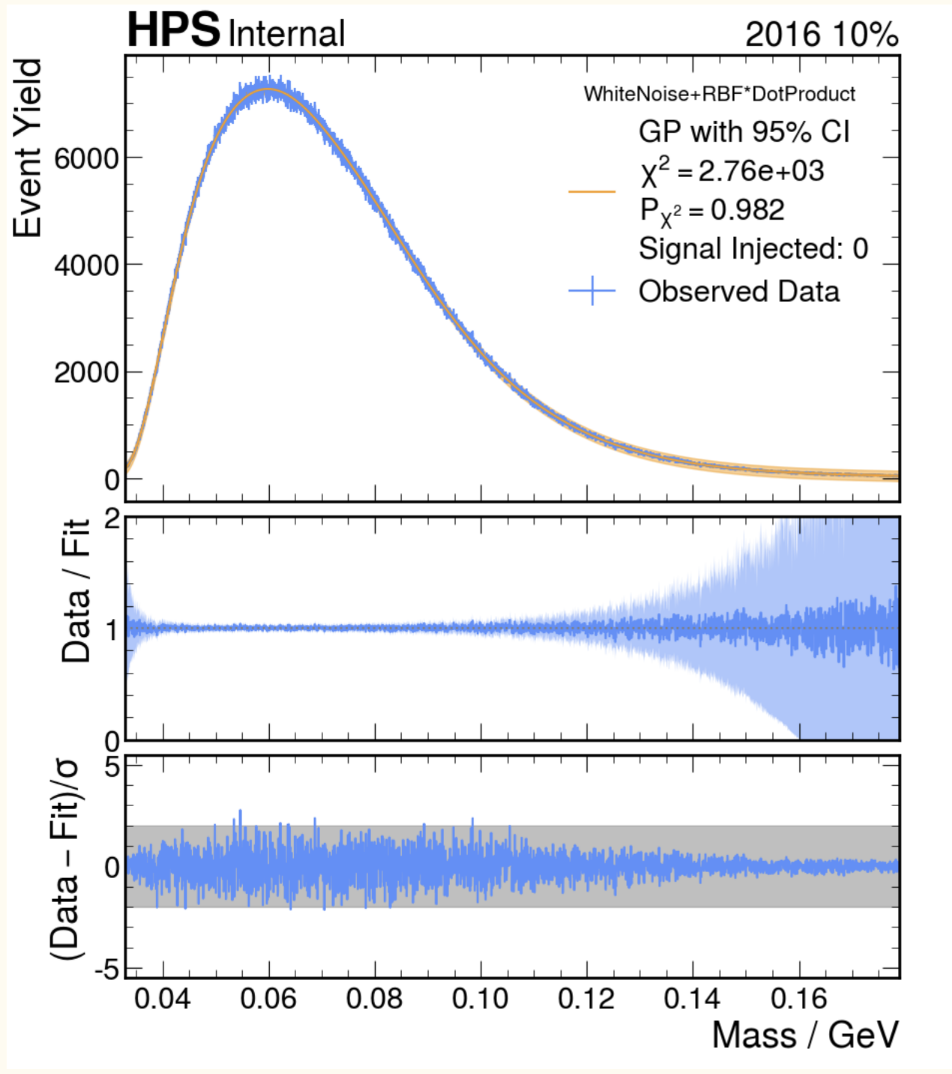
\includegraphics[width=0.96\linewidth]{appendix_figs/2016_10pct_whitenoisefit.png}
\caption{Historical global fit to the 2016 10\% sample using an RBF kernel multiplied
by a linear DotProduct kernel, with an added WhiteKernel term. The lower panel gives
the standardized residuals used in the original study to assess the fit. Although the
global description was acceptable, repeated use in the mass scan was unstable; the
figure therefore motivates the later local excluded-window construction and is not the
v3 Constant$\times$RBF background model.}
\label{fig:appendix-whitenoisefit-2016}
\end{figure}

\subsection{Historical piecewise fitting and kernel weighting}

The subsequent piecewise study trained a separate GP around each mass hypothesis,
withholding a central region from the background fit. Its kernel ensemble converted
the log marginal likelihood $\ell_k$ of each candidate $K_k$ to
\begin{equation}
w_k
=
\frac{\exp(\ell_k-\max_j\ell_j)}
{\sum_j\exp(\ell_j-\max_j\ell_j)}.
\end{equation}
A kernel was then sampled from these weights before producing a blind-region
prediction. This model-averaging experiment predates the frozen single-kernel
likelihood and is not used in the current scan. The sampling step made the inferred
background depend on both candidate-kernel likelihoods and a stochastic kernel choice;
the v3 analysis instead freezes one kernel family and validates its bounded length
scale with pseudoexperiments.

\begin{figure}[p]
\centering
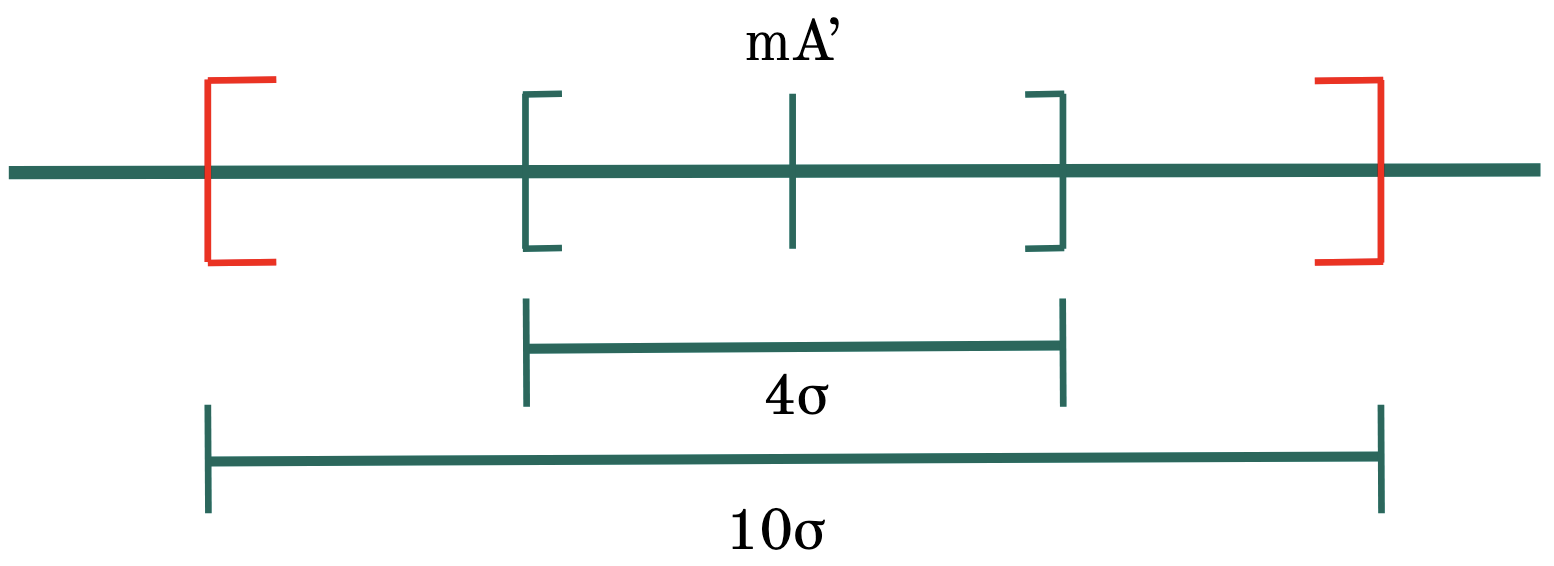
\includegraphics[width=0.94\linewidth]{appendix_figs/piecewise_diagram.png}
\caption{Schematic of the historical piecewise construction around one mass
hypothesis. A distinct GP was trained in a region of total width $10\,\sigma_m$ while
the central $5\,\sigma_m$ interval was hidden from that model and filled by
interpolation. These widths refer to the complete training section and blinded
interval in the early study; they should not be identified with the v3
$2.25\,\sigma_m$ half-width used for the blind and extraction window.}
\label{fig:appendix-piecewise-diagram}
\end{figure}

The associated signal-yield plot used a direct known-background Poisson construction,
not the profile-likelihood \CLs{} method used in v3. With fixed background expectation
$b$, observation $n$, and one-sided tail probability $\alpha$, that historical
construction was
\begin{equation}
\mu_{\mathrm{up}}
=
\frac{1}{2}F^{-1}_{\chi^2_{2(n+1)}}(1-\alpha),
\qquad
s_{\mathrm{up}}=\max(0,\mu_{\mathrm{up}}-b).
\end{equation}
The displayed study used $\alpha=0.05$. It is retained only to identify the
provenance of the old plot; no conversion between this 95\% construction and the v3
90\% CL result is performed.

\begin{figure}[p]
\centering
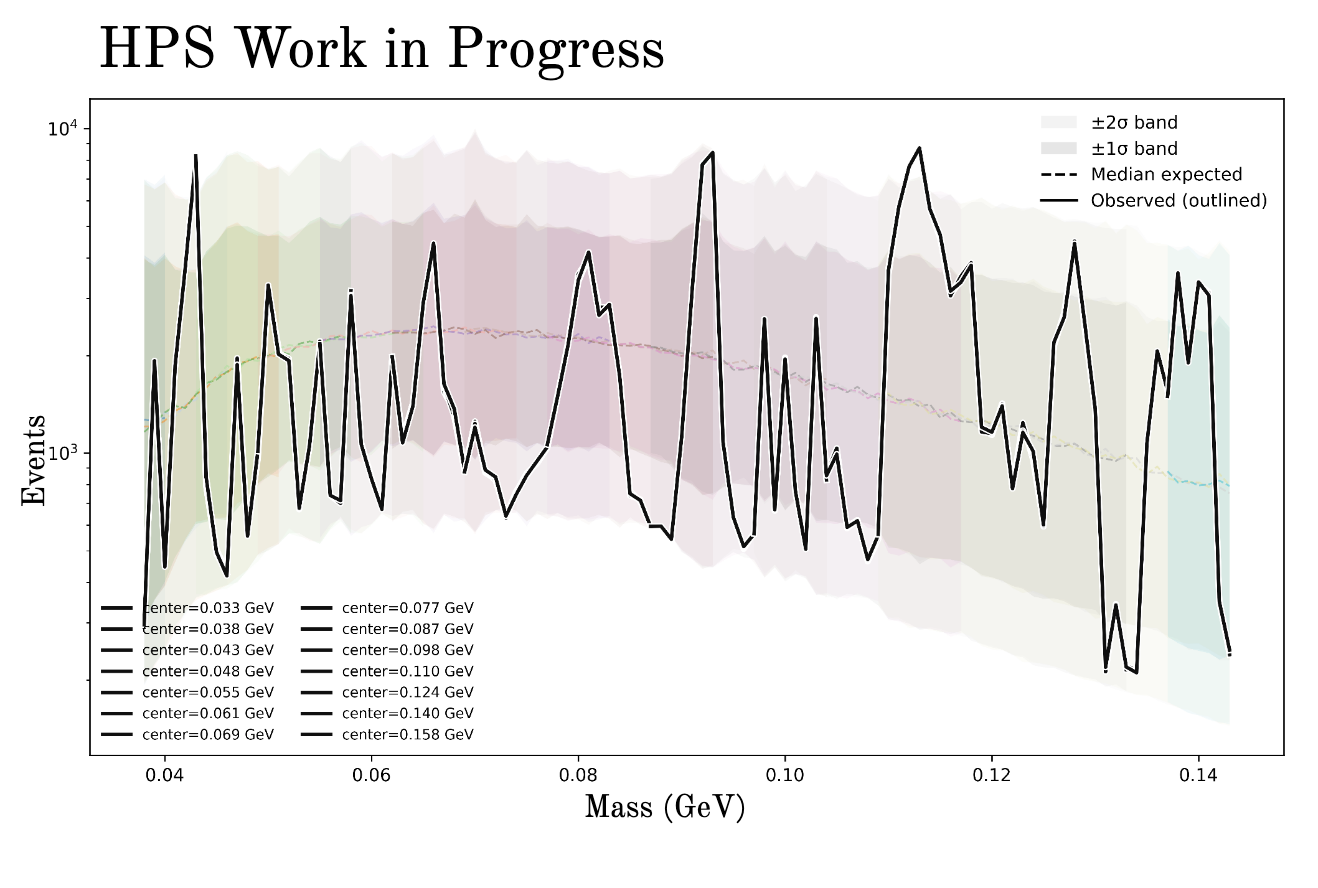
\includegraphics[width=0.94\linewidth]{appendix_figs/signal_yield_2016_10.png}
\caption{Historical signal-yield upper limit for the 2016 10\% sample obtained with
the piecewise GP construction. The shaded bands record the interval sizes used in that
study. Limits were computed with the direct known-background Poisson expression above
at $\alpha=0.05$, rather than the bounded profile-likelihood \CLs{} construction and
correlated GP-background nuisance parameters used in v3. The numerical curve is
therefore retained only to document the early method.}
\label{fig:appendix-signal-yield-2016}
\end{figure}

\subsection{Guard-band construction reference}
\label{app:guard-band-construction}

The guard-band construction considered during the 2015 closure campaign separated each
mass hypothesis into a central blind/extraction window, an adjacent band omitted from
both training and extraction, and outer GP-training sidebands. The central window
covered $|m-m_0|<1.64\,\sigma_m$, while the guard excluded
$1.64<|m-m_0|/\sigma_m<2.25$. The matched geometry study in
Section~\ref{subsec:guard-band-construction} selects the
$2.25\,\sigma_m$ blind/extraction window because it preserves the same training
protection while retaining the signal tails in the extraction likelihood.

\begin{figure}[p]
\centering
\graphicorplaceholder{0.96\linewidth}{guard_band_figs/guard_band_signal_leakage_cartoon.png}
\caption{Reference cartoon for the older guard-band construction. The red central
region is the $1.64\,\sigma_m$ blind/extraction window, the yellow bands are excluded
from GP training as a guard, and the green sidebands train the background. The study
tested whether preserving this separation reduced signal leakage into the sideband
fit. The v3 matched-geometry choice instead uses a $2.25\,\sigma_m$ blind/extraction
window, which protects the training sample while retaining the Gaussian signal tails
in the likelihood.}
\label{fig:appendix-guard-band-cartoon}
\end{figure}

\subsection{Exploratory cross-kernel closure}

An exploratory protocol fit the 2016 10\% spectrum with RBF and
\texttt{Matern32} kernels, generated 300 background-only toys from each fitted model,
and extracted each ensemble with the other kernel after Gaussian signal injection.
That study was designed to expose misspecification through pull bias. No frozen
coverage table or production-matched upper-limit export from this comparison is used
in v3, so it is not cited as evidence for the baseline kernel choice.
